\question{}

สมมติว่าเราต้องการสร้างรูปเรขาคณิตใหม่ โดยนำชิ้นส่วนจัตุรัสขนาด 1 ตารางหน่วยอย่างน้อย 1 ชิ้นมาประกอบกัน โดยมีเงื่อนไขดังต่อไปนี้
\begin{itemize}
    \item รูปเรขาคณิตใหม่จะต้องไม่มีชิ้นส่วนที่แยกจากกัน
        (ยกตัวอย่างเช่นรูป \textbf{(c)} \uline{ใช้ไม่ได้})
    \item ชิ้นส่วนจัตุรัสสองชิ้นที่แตะกันเฉพาะตำแหน่งมุม ถือว่าเป็นชิ้นส่วนที่แยกจากกัน
        (รูปตัวอย่าง \textbf{(d)} \uline{ใช้ไม่ได้})
    \item รูปเรขาคณิตใหม่จะต้องไม่มีรูหรือช่องว่างภายในรูปปิด 
        (ตัวอย่างเช่นรูป \textbf{(e)} \uline{ใช้ไม่ได้})
    \item รูปเรขาคณิตใหม่จะต้องมีทุกด้านยาว 1 หน่วยเท่านั้น 
        (เช่นรูป \textbf{(f)} หรือ \textbf{(g)} \uline{ใช้ไม่ได้} 
        เพราะมีบางด้านยาว 0.5 หน่วย หรือ 2 หน่วย)
\end{itemize}
\marginnote[-8\baselineskip]{%
    \centering
    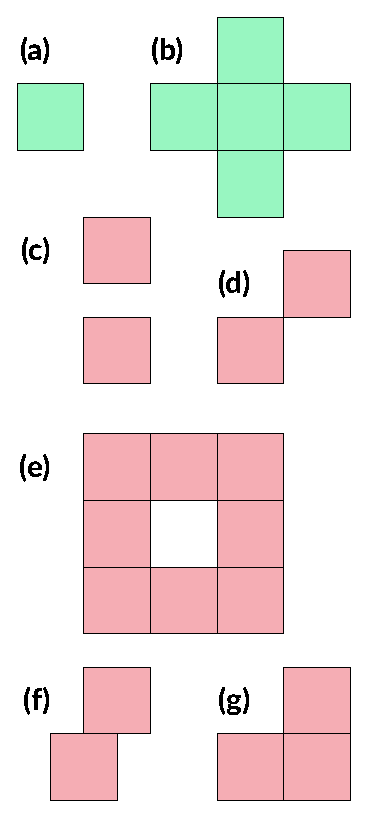
\includegraphics[width=0.70\linewidth]{figures/quickfire_central_audition_squaretiling.eps}
}

สังเกตว่า หากเรามีชิ้นส่วนจัตุรัส 1 ชิ้นพอดี หรือ 5 ชิ้นพอดี
(จากรูปตัวอย่าง \textbf{(a)} และ \textbf{(b)} ตามลำดับ) 
เราสามารถสร้างรูปเรขาคณิตที่สอดคล้องกับเงื่อนไขข้างต้นได้\;
อย่างไรก็ดี เรา\uline{ไม่สามารถ}สร้างรูปเรขาคณิตตามเงื่อนไขดังกล่าวได้เลย 
หากเรามีชิ้นส่วนจัตุรัสเพียง 2 หรือ 3 หรือ 4 ชิ้นเท่านั้น

จงหาจำนวนชิ้นส่วนจัตุรัสที่\hrsp\uline{มากที่สุด}{\hrsp}ที่\hrsp\uline{ไม่สามารถ}{\hrsp}นำมาประกอบเป็นรูปเรขาคณิตตามเงื่อนไขข้างต้นได้
